% mycsrf 'for beeing included' snippet template
%
% (c) Karsten Reincke, Frankfurt a.M. 2012, ff.
%
% This text is licensed under the Creative Commons Attribution 3.0 Germany
% License (http://creativecommons.org/licenses/by/3.0/de/): Feel free to share
% (to copy, distribute and transmit) or to remix (to adapt) it, if you respect
% how you must attribute the work in the manner specified by the author(s):
% \newline
% In an internet based reuse please link the reused parts to mycsrf.fodina.de
% and mention the original author Karsten Reincke in a suitable manner. In a
% paper-like reuse please insert a short hint to mycsrf.fodina.de and to the
% original author, Karsten Reincke, into your preface. For normal quotations
% please use the scientific standard to cite
%


%% use all entries of the bibliography

\subsubsection{Canorus ($\bigstar$$\bigstar$$\bigstar$)}

\acc{Canorus} ist ein Notensatzprogramm\footcite[vgl.][\nopage
wp]{Canorus2019a}, das gelegentlich auch als Nachgolger von \acc{NoteEdit}
gehandelt wird\footcite[vgl.][\nopage wp]{WpedCanorus2019a}. Die vorletzte
Version (0.7.2) aus dem Jahr 2015 wurde noch als \enquote{leichtgewichtige
Alternative} zu umfangreicheren Notensatzprogrammen
bezeichnet\footcite[vgl.][\nopage wp]{Kreussel2015a}. Der letzte Releasekandidat
(0.7.3) stammt vom Juni 2018\footcite[vgl.][\nopage wp]{Canorus2019b}. Reviews
der neueren Version stehen noch aus\footnote{Stand 01/2019}.

Die Homepage von \acc{Canorus} ist die
Sourceforge-Projektseite\footcite[vgl.][\nopage wp]{Canorus2019a}. Aktuell wird
das Programm nicht in allen Distributionen angeboten\footnote{so nicht in Ubuntu
18.04}; externe Pakete gibt es eher für ältere
Programmsammlungen\footcite[vgl.][\nopage wp]{RepoCanorus2019a}. Dies dürfte
einen einfachen Grund haben: Der -- von 2019 aus gesehene -- vorletzte
veröffentlichte Release-Candidat 0.7.2 stammte aus dem Jahr 2015, der letzte aus
2018\footcite[vgl.][\nopage wp]{Canorus2019b}. Über drei Jahre tat sich -- von
außen gesehen - in Sachen Weiterentwicklung also wenig. In der Opensourcewelt
ist das üblicherweise ein Zeichen dafür, dass das Projekt 'eingeschlafen'
ist\footnote{Auch vor 2015 soll es schon Unterbrechungen bei der Entwicklung
gegeben haben \cite[vgl.][\nopage wp]{UbuntuCanorus2014a}}. Die Veröffentlichung
vom Juni 2018 kam dann zu spät für z.B. die Ubuntu-LTS-Distribution
18.04\footnote{Long-Term-Service-Distributionen erscheinen seltener (bei Ubuntu
alle 2 Jahre), werden dafür aber länger mit Updates versorgt.}.
Gleichwohl sind wir sicher, dass das Programm in kommenden Distributionen wieder
aufgenommen wird.

So bleibt Anfang 2019 im Wesentlichen nur die Installation aus den Quellen,
falls man \acc{Canorus} nutzen will. Das sollte allerdings Programmierer und
Systemkenner nicht sehr herausfordern. Das Softwarepaket liefert eine
Readme-Datei mit, die für verschiedene Umgebungen die nötigen Befehle
auflistet\footnote{Für Ubuntu 18.04 konnten wir verifizieren, dass die
Kompilation einfach druchläuft, wenn man die geforderten Zusatzpakete -- wie
beschrieben -- installiert.}. Alternativ bleibt nur, auf die nächste
Distribution zu warten, die uns dieses Programm wieder ohne Eigenarbeit zur
Verfügung stellt.

\acc{Canorus} bietet keinen eigenen Notensatz im eigentlichen Sinne an. Dafür
nutzt es \acc{LilyPond} als Backend. Oder anders gesagt: \acc{Canorus} fungiert
als graphisches Frontend für die textuell arbeitenden \acc{LilyPond}. Das, was
man mit \acc{Canorus} erarbeitet, speichert es in einem eigenen
\acc{XML}-Format. Importieren kann man (gegenwärtig) nur \acc{MusicXML}- und
\acc{Midi}-Dateien, exportieren auch Graphiken und \acc{LilyPond-}Dateien.

Die Arbeitsteilung zwischen \acc{Canorus} und \acc{LilyPond} hat eine besondere
Konsequenz: was man am Bildschirm sieht, ist nicht das, was man als druckfertige
PDF-Datei erhält. Hier zunächst unsere Referenzkadenz, wie Canorus sie als PDF
generiert. Wie kaum anders zu erwarten, ähnelt sie sehr der 'puren'
\acc{LilyPond}-Ausgabe.

\begin{center}
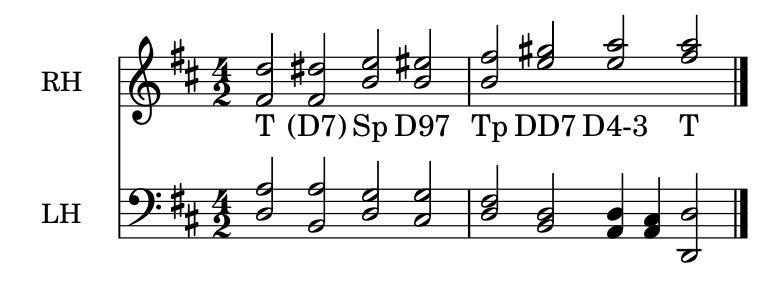
\includegraphics[width=0.8\textwidth]{frontends/cantrus/cadenca2-pdf.png}
\end{center}

Allerdings konnte der 4$\rightarrow$3 Vorhalt mit einer \Halb\ gegen zwei
gebundene \Vier\ im Bass offensichtlich nicht umgesetzt werden. Die
Funktionssymbole sind dagegen erkennbar -- ganz wie bei der Kadenz-I in der
reinen \acc{LilyPond}-Version\footnote{$\rightarrow$ S.
\pageref{LilyPondKadenzI}} -- als 'Liedtext' integriert worden. Hier wie da
gilt: ohne unsere kleine Zusatzbibliothek\footnote{$\rightarrow$ S.
\pageref{LilyPondFuncTheory}} können die Symbole der Funktionstheorie in einem
\acc{LilyPond}-Code nur in grober Form genutzt werden.

Dieser Ausgabe steht graphisch eine leicht anders gestaltete Eingabe gegenüber:

\begin{center}
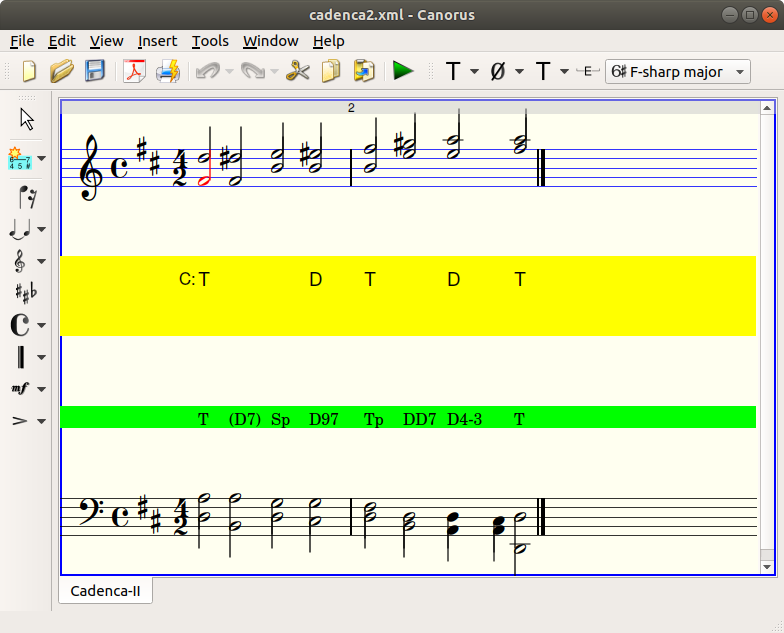
\includegraphics[width=0.8\textwidth]{frontends/canorus/cadenca2-canorus}
\end{center}

Man erkennt auf der linken Seite die Konzexte, die für Spezialeingaben zu
aktivieren sind. Der Modus zur Eingabe von Noten wird über das Menu aktiviert.
Oben in der Liste erscheinen die konkreten Ausformungen. Letztlich klickt man
mit der Maus dort in das Notensystem, wo die gewünschte Note erscheinen soll;
Vorzeichen werden zuvor mit \texttt{+} oder \texttt{-} aktiviert. \acc{Canorus}
ist also recht intuitiv zu bedienen. Darum fällt es nur bedingt ins Gewicht, dass
das Handbuch bei der manuelle Installation aus den Quellen heraus nicht mit
kompiliert wird\footnote{\ldots und bis dato auch nicht im Netz zu finden ist}.

Für die Eingabe von 'Liedtext' stellt \acc{Canorus} einen besonderen Modus
bereit\footnote{der untere, grüne Bereich zwischen den Notenliniensystemen}, den
man ebenfalls im linken Randbereich aktiviert und dann über Maus und Tastatur
bedient.

Außer dem Textmodus möchte \acc{Canorus} auch noch einen Modus zur
Harmonieanalyse\footnote{der obere, gelbe Bereich zwischen den
Notenliniensystemen} bereitstellen. In diesem Modus kann man -- wie es unser
Bild zeigt -- in der oberen Programmleiste Funktionssymbole auswählen und unter
bestimmte Noten einfügen. Tatsächlich versucht \acc{Canorus} sogar, den
entsprechenden Akkord zu analysieren.

Damit verfolgt \acc{Canorus} einen vielversprechenden Ansatz, der über den
anderer Notensatzsysteme hinausgeht. Gleichwohl ist das Ergebnis aus drei
Gründen noch nicht produktiv nutzbar: Zum ersten werden \acc{Canorus} eigenen
Analysesymbole nicht mit gedruckt und exportiert. Zum zweiten löst die Nutzung
dieses Modus noch viele Programmabstürze aus. Und drittens kann man in diesem
Modus noch keine Funktionsparallelen, keine Gegenklänge und keine
Doppeldominaten ausdrücken\footnote{Die angebotene Alternative der
Zwischendominante funktioniert nicht zuverlässig.}. Darum ist dieses sehr
innovative Verfahren für den heutigen Musikwissenschaftler praktisch nicht
verwendbar.

Der \acc{LilyPond}-Code, den \acc{Canorus} exportiert, kann dagegen schon heute
gut weiterverarbeitet werden. Er ist -- sofern man auf die eigene und die
\acc{Canorus}-Harmonieanalyse verzichtet -- gut strukturiert, lesbar und
reproduzierbar\footnote{$\rightarrow$ S.\pageref{ExportVerifikation}}
korrekt\footnote{Aus Platzgründen verzichten wir auf den erneuten Abdruck des
\acc{LilyPond}-Codes}. Ohne eine textuelle Nachbearbeitung wird er aber für den
Musikwissenschaftler nur bedingt sinnvoll sein.

So geben wir dem Programm 3 von 5 Sternen: In Maßen kann es jetzt bereits als
Frontend für \acc{LilyPond} verwendet werden, es ist vielversprechend, wird aktuell
gepflegt und erfüllt die Basisanforderungen. Als $\beta$-Version ist es aber von
der Funktionalität und von der Stabilität her ebenso noch begrenzt, wie vom Handling
her. Praktisch wird \acc{Canorus} momentan allenfalls für den
Musikwissenschaftler als \acc{LilyPond}-Frontend in Frage kommen, der bereits mit
\acc{Canorus} vertraut ist.


% this is only inserted to eject fault messages in texlipse
%\bibliography{../bib/literature}
